\documentclass[11pt]{article}
\usepackage[a4paper,margin=1in]{geometry}
\usepackage[T1]{fontenc}
\usepackage[utf8]{inputenc}
\usepackage{newtxtext,newtxmath}
\usepackage{setspace}
\usepackage{graphicx}
\usepackage{booktabs}
\usepackage{longtable}
\usepackage{array}
\usepackage{float}
\usepackage{caption}
\usepackage{hyperref}
\usepackage{titlesec}
\usepackage{fancyhdr}
\setstretch{1.15}
\pagestyle{fancy}
\fancyhf{}
\fancyhead[L]{Healthcare NLP ADR Project}
\fancyfoot[C]{\thepage}
\setlength{\headheight}{14pt}
\titleformat{\section}{\large\bfseries}{\thesection.}{0.5em}{}
\titleformat{\subsection}{\normalsize\bfseries}{\thesubsection.}{0.5em}{}
\title{Adverse Drug Reaction Detection from Biomedical Text: A Comprehensive MS-Level NLP Project Report}
\author{Kamrul Hasan}
\date{April 2026}
\begin{document}
\maketitle
\tableofcontents
\newpage

\section{Abstract}

Adverse Drug Reactions (ADRs) remain a persistent healthcare safety challenge because critical evidence is often embedded in free text rather than structured fields. This project develops and evaluates a complete NLP pipeline for sentence-level ADR classification using a public benchmark dataset, with two modeling tracks: classical machine learning (ML) and transformer-based fine-tuning. The study is implemented on ADE Corpus V2, a biomedical case-report corpus containing 23,516 labeled sentences. The project objective is not only to maximize classification quality, but also to characterize data behavior through exploratory data analysis (EDA), establish reproducible technical methodology, tune model families under comparable conditions, and interpret model outcomes in a clinically meaningful way.


The final pipeline includes dataset preparation, text normalization, TF-IDF feature extraction, hyperparameter tuning for Logistic Regression, Linear SVM, Random Forest, and Naive Bayes, and a fine-tuned BioClinicalBERT configuration. Evaluation uses Accuracy, Precision, Recall, F1, ROC-AUC, PR-AUC, and confusion-matrix analysis. On full classical evaluation, Linear SVM achieved the strongest test performance (F1 = 0.8440, ROC-AUC = 0.9600, PR-AUC = 0.9201). BioClinicalBERT fine-tuning (sampled training run for computational feasibility) achieved strong but lower values on this run (F1 = 0.8175, ROC-AUC = 0.9536, PR-AUC = 0.8953), indicating robust contextual performance but also sensitivity to training budget.


The report provides deep interpretation of class imbalance, sentence-length effects, lexical signal distribution, model trade-offs, and practical deployment implications for pharmacovigilance contexts. The final contribution is an end-to-end, reproducible, MS-level ADR detection framework with transparent experimentation, artifact generation, and clear pathways for scaling to thesis-grade extensions.


\section{Keywords}

Adverse Drug Reaction, Pharmacovigilance, Biomedical NLP, Text Classification, TF-IDF, BioClinicalBERT, Explainable Evaluation, Healthcare AI


\section{Introduction}

Textual clinical evidence is one of the richest but least structured sources of drug safety information. Adverse Drug Reactions are discussed in case reports, physician notes, and narrative clinical communication, often with variable language, sparse standardization, and ambiguous temporal framing. As a result, manual review is expensive and delayed, while automated systems face difficult linguistic and class-imbalance conditions.


This project addresses ADR sentence classification as a practical and educationally rigorous graduate-level problem. The scope includes building a production-like data and modeling pipeline, evaluating both traditional and modern NLP methods, and producing interpretable analyses suitable for a graduate report. Rather than treating model training as an isolated coding task, this work emphasizes methodological discipline: explicit problem framing, reproducible preprocessing, controlled hyperparameter experimentation, artifact-driven interpretation, and grounded conclusions.


To make the task concrete, consider the sentence: "Developed facial swelling shortly after first dose of antibiotic." A human reader would immediately recognize a drug-event relationship, and the model should assign it ADR = 1. In contrast, the sentence "Medication tolerated well with no adverse reactions" should be assigned ADR = 0 because it explicitly states the absence of side effects.


The report is structured in paper form (Abstract, Introduction, Data, EDA, Methodology, Experiments, Results, Discussion, Conclusion) and intentionally excludes a literature review per project instruction.


\section{Problem Statement and Project Definition}

\subsection{Problem Statement}

Given a sentence from biomedical text, predict whether it contains an adverse drug reaction signal.


Formally, let each input sentence be $x_i$ and binary label $y_i \in {0,1}$ where:


\begin{itemize}
  \item $y_i = 1$: ADR-related sentence
  \item $y_i = 0$: non-ADR sentence
\end{itemize}

The objective is to learn a classifier $f(x)$ that generalizes well to unseen biomedical narrative text while preserving clinically meaningful recall and precision balance. For example, if the model sees "Nausea and dizziness started two days after ibuprofen," it should map the text to the ADR class because the symptoms are temporally connected to the drug mention.


\subsection{Why This Problem Matters}


\begin{itemize}
  \item Missed ADR signals delay safety awareness and increase patient risk. For example, a case report may mention "persistent cough after lisinopril" only once; if that sentence is overlooked, the event may never reach a safety analyst.
  \item Narrative data volume is too large for purely manual review.
  \item High-quality sentence classification can act as an upstream filter for downstream extraction, monitoring, or alert systems.
\end{itemize}

\subsection{What We Are Going To Do}

This project executes the following plan:


\begin{enumerate}
  \item Construct a standardized ADR dataset from a public benchmark.
  \item Perform EDA to understand class balance, text lengths, lexical behavior, and modeling implications.
  \item Build classical baselines with TF-IDF and tuned classifiers.
  \item Fine-tune BioClinicalBERT as the transformer track.
  \item Compare all models across consistent metrics.
  \item Interpret outcomes with graph- and table-based evidence.
  \item Provide reproducible artifacts and clear next-step recommendations.
\end{enumerate}

\subsection{Research Questions}

\begin{enumerate}
  \item How well do tuned classical ML models perform on ADR sentence classification?
  \item Under practical MS-level compute constraints, does BioClinicalBERT outperform classical baselines?
  \item What data characteristics (imbalance, sentence length, lexical cues) influence model behavior?
  \item Which model profile is preferable for deployment: highest recall, highest precision, or best balanced F1/PR-AUC?
\end{enumerate}

\section{Project Scope, Assumptions, and Deliverables}

\subsection{Scope}

\begin{itemize}
  \item In scope: binary sentence classification for ADR detection from biomedical text.
  \item In scope: end-to-end reproducible pipeline with generated EDA and result artifacts.
  \item In scope: classical and transformer comparison.
  \item Out of scope: relation extraction, temporal relation modeling, and literature review chapter.
\end{itemize}

\subsection{Assumptions}

\begin{itemize}
  \item ADE labels are treated as reliable benchmark supervision. A sentence such as "Developed severe rash after taking amoxicillin" is presumed to be a positive label because the dataset annotations define it as ADR-related.
  \item Sentence-level classification is an acceptable approximation of ADR evidence detection.
  \item BioClinicalBERT run uses sampled training for computational feasibility in current environment.
\end{itemize}

\subsection{Deliverables}

\begin{itemize}
  \item Processed dataset and data pipeline.
  \item Trained baseline and transformer result summaries.
  \item EDA figures/tables and model comparison artifacts.
  \item Comprehensive paper-style report.
\end{itemize}

\section{Dataset Description}

\subsection{Data Source}

\begin{itemize}
  \item Dataset: ade-benchmark-corpus/ade\_corpus\_v2
  \item Configuration: Ade\_corpus\_v2\_classification
  \item Prepared CSV: data/processed/ade\_corpus\_v2\_classification.csv
\end{itemize}

\subsection{Label Definition}

\begin{itemize}
  \item ADR (1): sentence contains adverse drug effect evidence. Example: "After starting antidepressant, the patient reported severe insomnia and nausea."
  \item No ADR (0): sentence does not contain adverse drug effect evidence. Example: "The patient improved after routine follow-up with no complications."
\end{itemize}

\subsection{Dataset Size and Splits}

\begin{itemize}
  \item Total rows: 23,516
  \item Train/Validation/Test: 16,461 / 3,527 / 3,528 (classical track)
  \item BioClinicalBERT sampled run: 3,000 / 1,000 / 1,000
\end{itemize}

\subsection{Class Distribution}

From generated dataset statistics:


\begin{itemize}
  \item ADR rows: 6,821
  \item No ADR rows: 16,695
  \item ADR ratio: 0.2901 (approximately 29\%)
\end{itemize}

This imbalance motivates metric emphasis on F1 and PR-AUC rather than raw accuracy alone.


\begin{figure}[H]
\centering
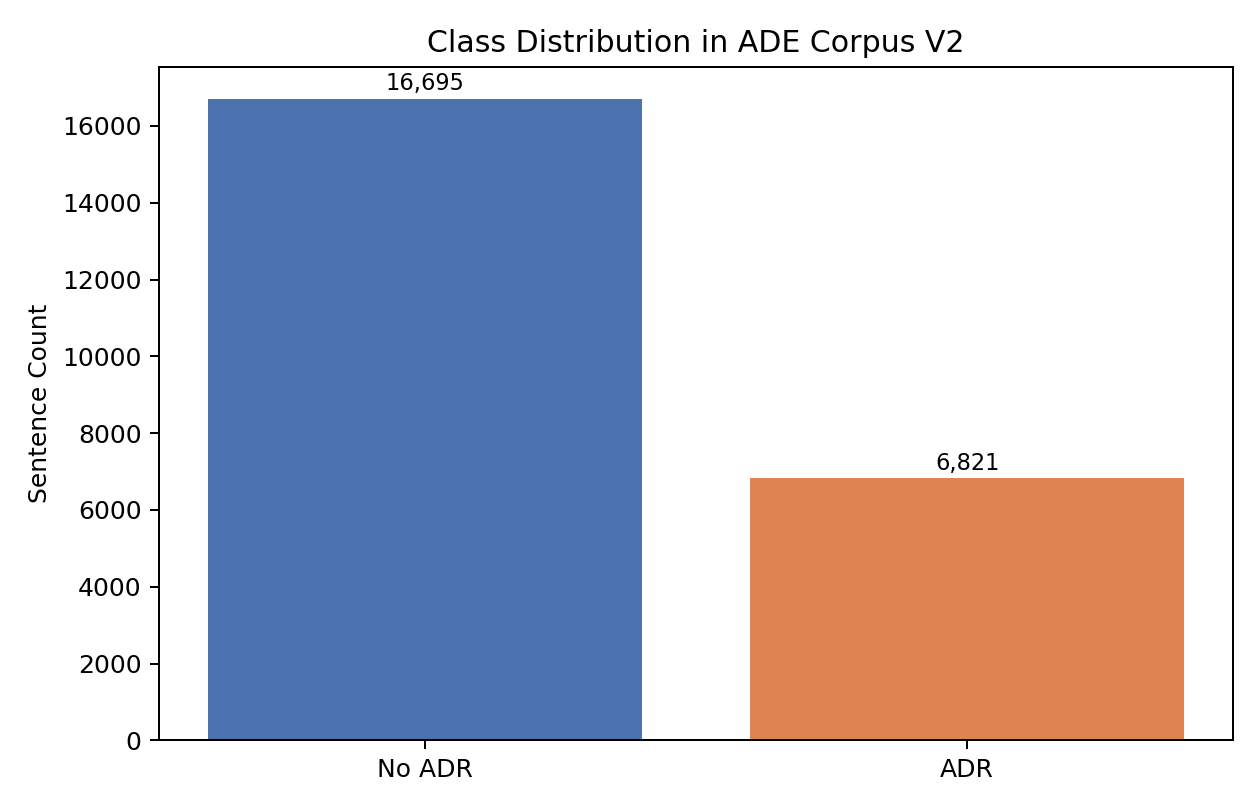
\includegraphics[width=0.9\linewidth]{artifacts/fig01_label_distribution.png}
\caption{Figure 1. Class distribution}
\end{figure}


**Interpretation:** The dataset is moderately imbalanced toward non-ADR sentences. A naive classifier biased toward majority class could overstate performance via accuracy, so robust evaluation must prioritize minority sensitivity. In plain language, a model that simply says "no ADR" for every sentence would already be correct about 71 percent of the time, but it would be useless for safety monitoring because it would miss the actual reactions.


\section{Exploratory Data Analysis (EDA)}

\subsection{Text Length Characteristics}

Dataset-wide summary:


\begin{itemize}
  \item Mean words per sentence: 18.54
  \item Median words per sentence: 17
  \item Standard deviation: 9.07
  \item Interquartile range: 12 to 23 words
  \item Maximum observed length: 135 words
\end{itemize}

Per-class mean length:


\begin{itemize}
  \item ADR: 20.56 words
  \item No ADR: 17.71 words
\end{itemize}

\begin{figure}[H]
\centering
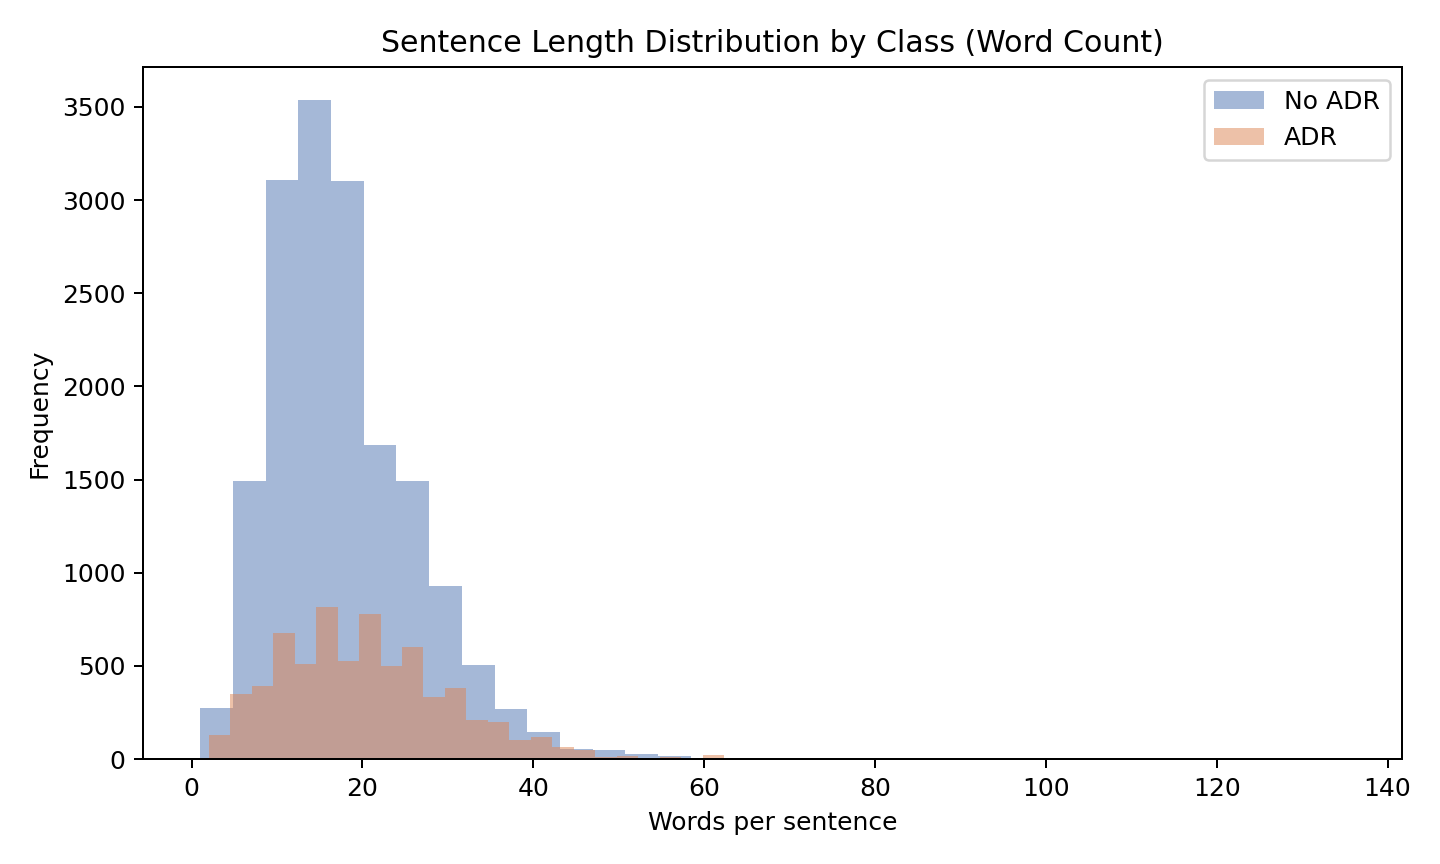
\includegraphics[width=0.9\linewidth]{artifacts/fig02_word_length_hist.png}
\caption{Figure 2. Word-count histogram by class}
\end{figure}


\begin{figure}[H]
\centering
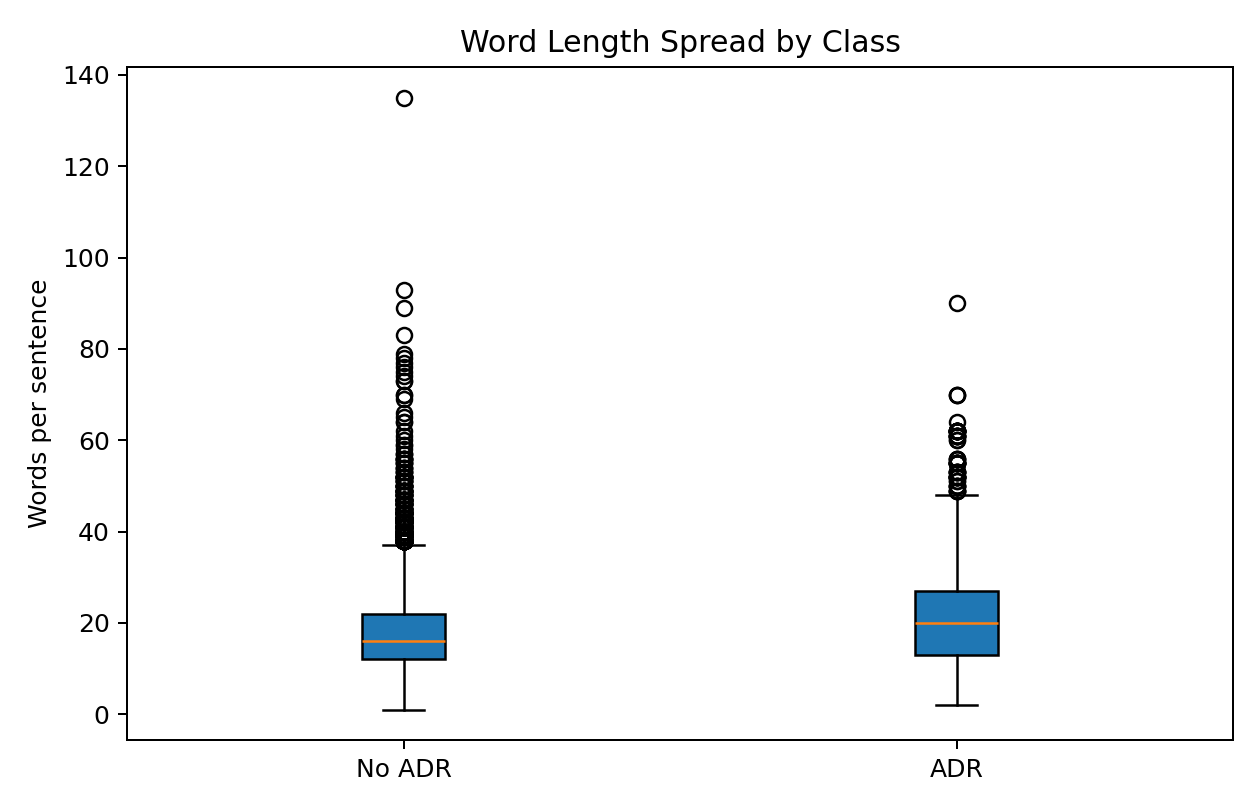
\includegraphics[width=0.9\linewidth]{artifacts/fig03_word_length_boxplot.png}
\caption{Figure 3. Word-count boxplot by class}
\end{figure}


**Interpretation:** ADR sentences are, on average, longer than non-ADR sentences. This may reflect richer event description structure (drug mention, symptom description, severity cue, and narrative context in the same sentence). For example, a sentence like "She developed a severe headache and blurred vision after the second dose" contains multiple clues that help classification. Longer sequences can favor contextual encoders, but TF-IDF also benefits because longer sentences increase feature evidence.


\subsection{Lexical Signal Analysis}

Top ADR-favoring TF-IDF terms (difference analysis) include: induced, associated, developed, severe, toxicity, syndrome, hypersensitivity.


Top non-ADR-favoring terms include: showed, diagnosis, infection, normal, results, complete, improvement.


This distinction is exported in:


\begin{itemize}
  \item artifacts/table\_discriminative\_tfidf\_terms.csv
\end{itemize}

Top frequency tables are exported in:


\begin{itemize}
  \item artifacts/table\_top\_terms\_adr.csv
  \item artifacts/table\_top\_terms\_no\_adr.csv
\end{itemize}

**Interpretation:** The discriminative lexicon aligns with biomedical semantics. ADR class terms are event-oriented and adverse-outcome oriented, while non-ADR terms often reflect routine clinical progression, assessment, and treatment management language. In practical terms, words such as "toxicity" or "hypersensitivity" are strong ADR clues, whereas words such as "improvement" or "diagnosis" more often appear in general clinical description. This explains why linear TF-IDF models remain highly competitive in this domain.


\subsection{EDA Implications for Modeling}

\begin{enumerate}
  \item Imbalance requires robust minority-aware metrics and potentially class weighting.
  \item Moderate sentence lengths suggest both bag-of-ngrams and transformer windows are suitable.
  \item Strong lexical cues indicate linear models can capture significant signal.
  \item Remaining context ambiguity motivates transformer experimentation.
\end{enumerate}

\section{Methodology}

\subsection{End-to-End Pipeline}

The pipeline includes:


\begin{enumerate}
  \item Dataset ingestion and schema validation.
  \item Text normalization and preparation.
  \item Split strategy and reproducible random seeds.
  \item Baseline model training with hyperparameter search.
  \item Transformer fine-tuning with controlled subset for feasibility.
  \item Metric computation and artifact generation.
  \item Comparative analysis and report generation.
\end{enumerate}

\subsection{Preprocessing Strategy}

Applied preprocessing includes:


\begin{itemize}
  \item Lowercasing
  \item URL and non-alphanumeric cleanup
  \item whitespace normalization
\end{itemize}

No aggressive stopword removal or stemming was applied in transformer training. Classical models rely on TF-IDF tokenization and n-gram settings. Example: the sentence "Nausea and dizziness started two days after ibuprofen" is normalized to lowercase, punctuation is removed, and the resulting cleaned text is easier for vectorizers to represent consistently.


\subsection{Feature Engineering (Classical Track)}

Primary representation: TF-IDF vectors with selectable unigram/bigram range.


Example: in the sentence "severe rash after amoxicillin," TF-IDF gives weight to terms such as "rash" and "amoxicillin" because they help distinguish ADR from non-ADR text.


Rationale:


\begin{itemize}
  \item Efficient for medium-sized corpora.
  \item Strong interpretability through term weights.
  \item Effective with linear learners for sparse text classification.
\end{itemize}

\subsection{Modeling Tracks}

\subsubsection{Classical ML Models}

\begin{itemize}
  \item Logistic Regression
  \item Linear SVM
  \item Random Forest
  \item Multinomial Naive Bayes
\end{itemize}

\subsubsection{Transformer Model}

\begin{itemize}
  \item Base model: emilyalsentzer/Bio\_ClinicalBERT. This is a BERT-family language model already pretrained on biomedical and clinical text, so it has stronger domain vocabulary than a general-purpose encoder.
  \item Head: sequence classification (2 labels). The head is the final classifier layer that turns a text embedding into ADR vs no-ADR probabilities.
  \item Fine-tuned using Hugging Face Trainer. In practice, this means the model parameters are updated on the ADR task instead of being used only as a frozen feature extractor.
\end{itemize}

\subsection{Evaluation Metrics}

Primary metrics:


\begin{itemize}
  \item Precision
  \item Recall
  \item F1-score
  \item PR-AUC
\end{itemize}

Secondary metrics:


\begin{itemize}
  \item Accuracy
  \item ROC-AUC
\end{itemize}

Diagnostic metric:


\begin{itemize}
  \item Confusion matrix
\end{itemize}

Why this set: ADR detection is minority-sensitive; PR-AUC and F1 better capture quality under imbalance than accuracy alone. For example, a model that finds many ADRs but produces too many false alarms may have high recall but low precision; F1 balances the two.


\section{Technical Setup and Hyperparameters}

\subsection{Environment and Tooling}

\begin{itemize}
  \item Language: Python
  \item Data/ML libraries: pandas, numpy, scikit-learn
  \item Transformer stack: transformers, datasets, torch, accelerate
  \item Plotting: matplotlib
\end{itemize}

\subsection{Split and Reproducibility Parameters}

\begin{itemize}
  \item Classical split ratio: 70/15/15
  \item Random seed: 42
  \item Stratified splitting by label
\end{itemize}

\subsection{Classical Model Hyperparameter Search Space}

\begin{table}[H]
\centering
\begin{tabular}{lc}
\toprule
Model & Hyperparameters Tuned \\
\midrule
Logistic Regression & C in \{0.5, 1.0, 2.0\}; ngram range in \{(1,1), (1,2)\} \\
Linear SVM & C in \{0.5, 1.0, 2.0\}; ngram range in \{(1,1), (1,2)\} \\
Random Forest & max\_depth in \{None, 50\}; min\_samples\_split in \{2, 5\} \\
Naive Bayes & alpha in \{0.3, 1.0, 2.0\} \\
\bottomrule
\end{tabular}
\end{table}


Shared vectorizer setup includes sublinear TF and high max\_features cap for broad lexical coverage.


\subsection{BioClinicalBERT Fine-Tuning Parameters (Executed Run)}

\begin{table}[H]
\centering
\begin{tabular}{lc}
\toprule
Parameter & Value \\
\midrule
Epochs & 1 \\
Learning rate & 2e-5 \\
Max length & 256 \\
Train batch size & 8 \\
Eval batch size & 16 \\
Train sample size & 3000 \\
Eval sample size & 1000 \\
Weight decay & 0.01 \\
Best-model criterion & F1 \\
\bottomrule
\end{tabular}
\end{table}


\subsection{Notes on Practical Constraints}

BioClinicalBERT was intentionally run on a sampled subset to maintain tractable wall-clock time on CPU-bound environment. This is appropriate for MS-level prototyping, but full-data training is recommended for final thesis-level benchmarking.


\section{Experimental Results}

\subsection{Full Model Comparison}

\begin{figure}[H]
\centering
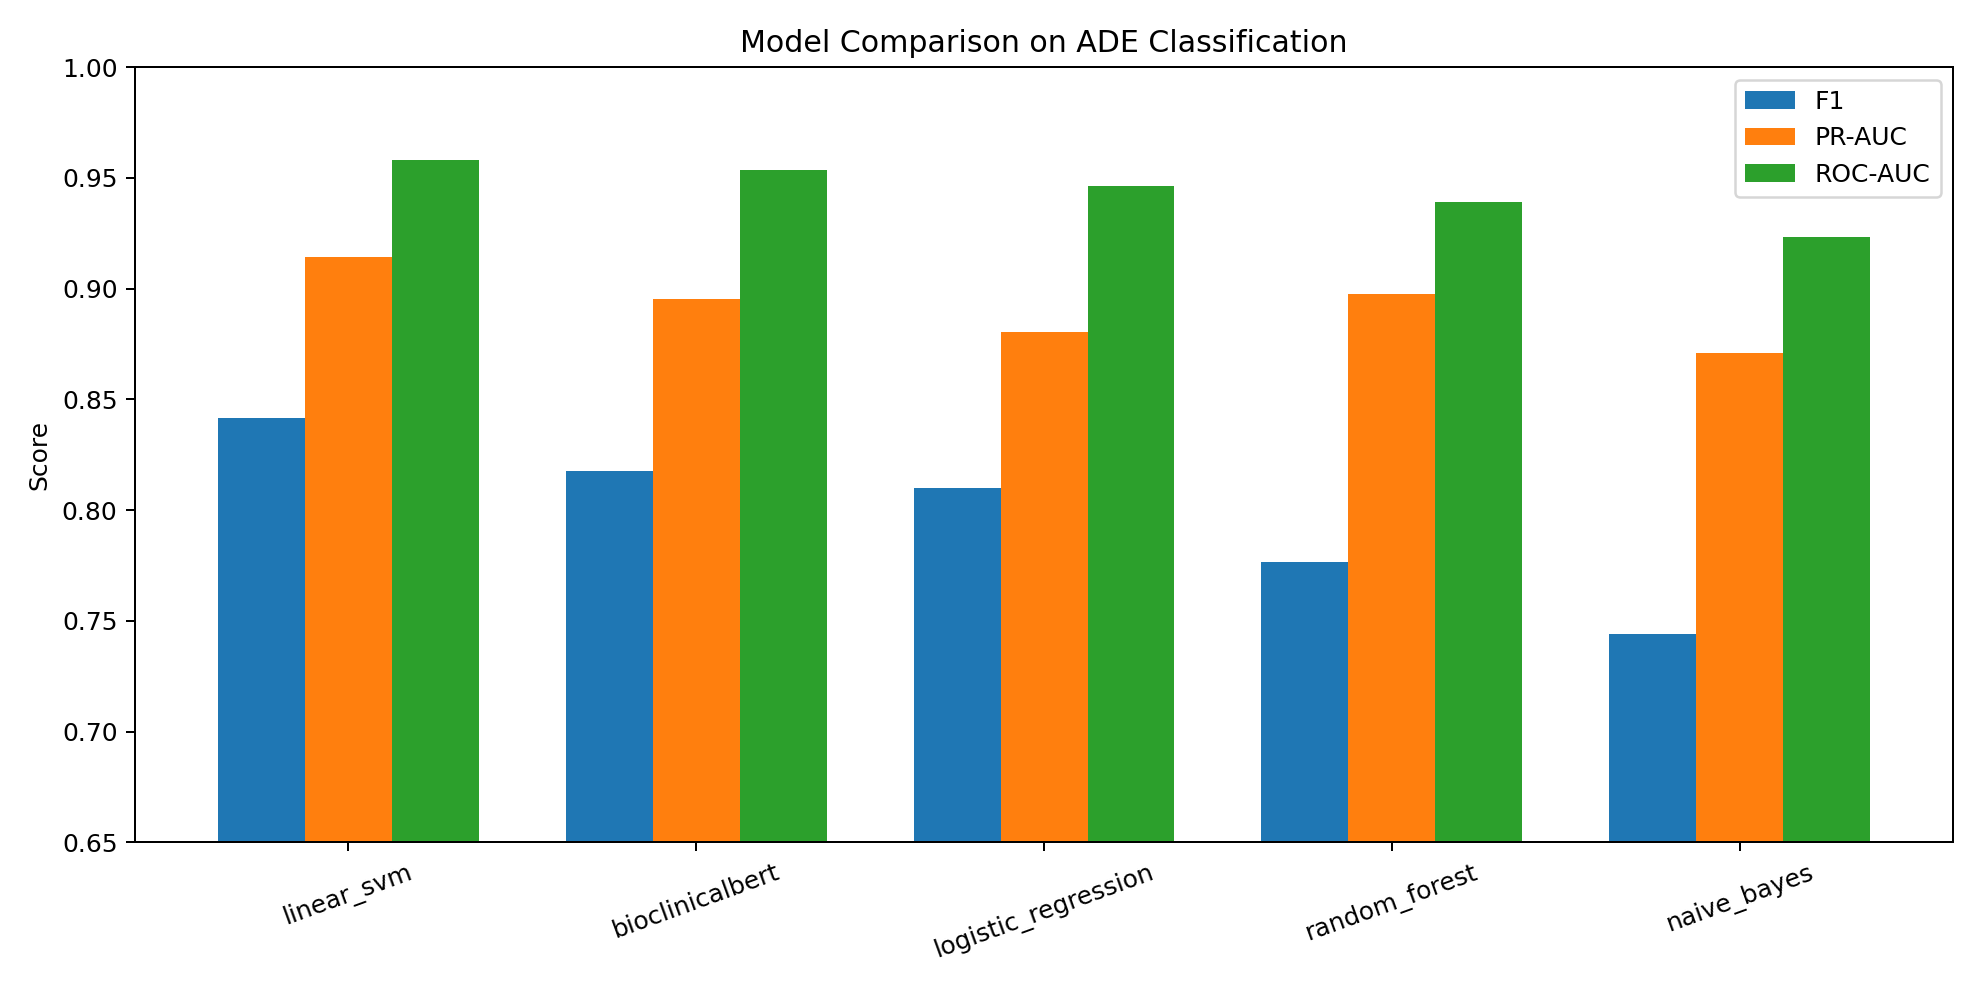
\includegraphics[width=0.9\linewidth]{artifacts/fig04_model_metric_comparison.png}
\caption{Figure 4. Comparative metric chart}
\end{figure}


Numerical summary (test split):


\begin{table}[H]
\centering
\begin{tabular}{lccccc}
\toprule
Model & F1 & Precision & Recall & ROC-AUC & PR-AUC \\
\midrule
Linear SVM & 0.8417 & 0.8036 & 0.8837 & 0.9581 & 0.9142 \\
Logistic Regression & 0.8101 & 0.7648 & 0.8612 & 0.9462 & 0.8804 \\
Random Forest & 0.7767 & 0.8850 & 0.6921 & 0.9392 & 0.8976 \\
Naive Bayes & 0.7439 & 0.8820 & 0.6432 & 0.9232 & 0.8710 \\
BioClinicalBERT (sampled run) & 0.8175 & 0.8116 & 0.8235 & 0.9536 & 0.8953 \\
\bottomrule
\end{tabular}
\end{table}


**Interpretation:**


\begin{enumerate}
  \item Linear SVM is strongest overall by F1 and PR-AUC in this project run.
  \item Logistic Regression remains competitive but slightly below SVM.
  \item Random Forest and Naive Bayes show high precision but noticeably lower recall, indicating under-capture of ADR positives.
  \item BioClinicalBERT shows strong discriminative quality, but did not exceed SVM under sampled, short-epoch training settings.
\end{enumerate}

\subsection{Best Classical Model Deep Dive (Linear SVM)}

Final best-baseline metrics from full split evaluation:


\begin{itemize}
  \item Accuracy: 0.9059
  \item Precision: 0.8127
  \item Recall: 0.8778
  \item F1: 0.8440
  \item ROC-AUC: 0.9600
  \item PR-AUC: 0.9201
\end{itemize}

Confusion matrix:


\begin{itemize}
  \item True Negative: 2298
  \item False Positive: 207
  \item False Negative: 125
  \item True Positive: 898
\end{itemize}

\begin{figure}[H]
\centering
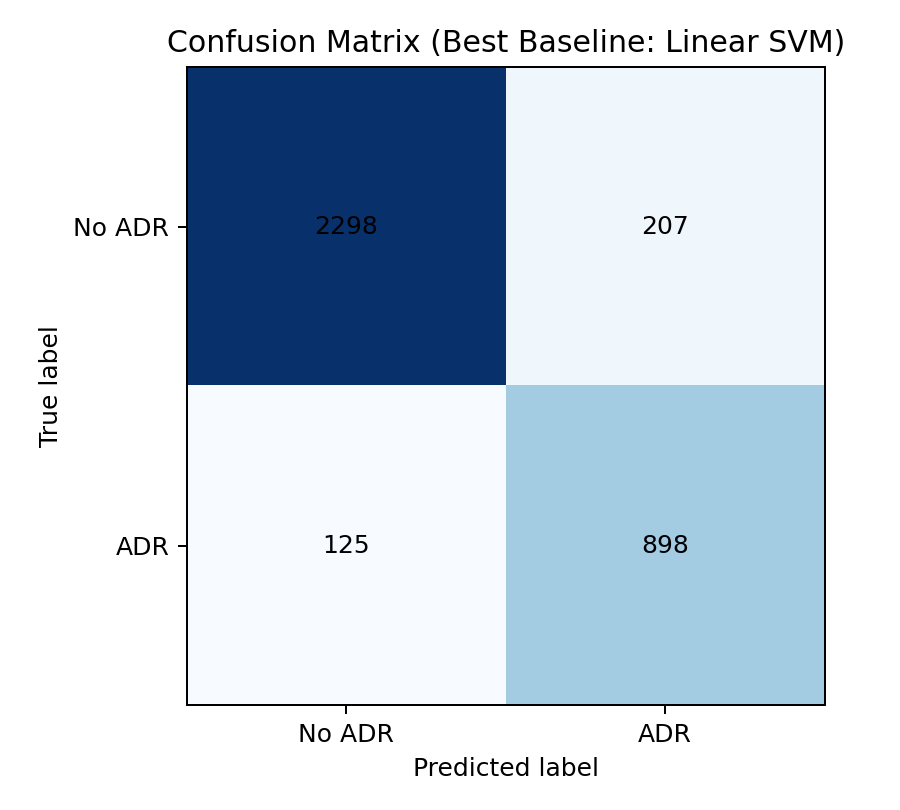
\includegraphics[width=0.9\linewidth]{artifacts/fig05_confusion_matrix_baseline.png}
\caption{Figure 5. Confusion matrix (Linear SVM)}
\end{figure}


**Interpretation:** False negatives are lower than false positives in absolute terms relative to class support, supporting a recall-oriented profile appropriate for safety screening. In pharmacovigilance pre-screening, this is usually preferable to precision-only optimization.


\subsection{BioClinicalBERT Run Analysis}

Validation:


\begin{itemize}
  \item Accuracy: 0.8980
  \item Precision: 0.8221
  \item Recall: 0.8333
  \item F1: 0.8277
  \item ROC-AUC: 0.9528
  \item PR-AUC: 0.8940
\end{itemize}

Test:


\begin{itemize}
  \item Accuracy: 0.9000
  \item Precision: 0.8116
  \item Recall: 0.8235
  \item F1: 0.8175
  \item ROC-AUC: 0.9536
  \item PR-AUC: 0.8953
\end{itemize}

**Interpretation:** The model generalizes stably from validation to test under sampled splits, showing low overfitting at this configuration. However, it likely remains undertrained compared to its potential due to one epoch and reduced train set.


\section{Discussion}

\subsection{Why Classical SVM Won in This Run}

Several factors explain SVM leadership in this setup:


\begin{enumerate}
  \item Strong lexical separability in biomedical ADR language.
  \item Large full classical training split versus sampled transformer training.
  \item Carefully tuned linear hyperparameters.
  \item Sparse linear models often excel on sentence-level clinical classification where class cues are explicit.
\end{enumerate}

\subsection{Transformer Strengths Still Evident}

Despite not ranking first here, BioClinicalBERT achieved high ROC-AUC and PR-AUC, demonstrating rich contextual sensitivity. With full-data fine-tuning, additional epochs, and hardware acceleration, it is plausible that transformer performance could match or exceed current baseline leaders.


\subsection{Metric Trade-Offs and Deployment View}

For ADR safety triage:


\begin{itemize}
  \item Higher recall reduces missed adverse signals.
  \item Moderate precision can be acceptable if downstream human review exists.
  \item PR-AUC provides realistic insight in imbalanced operational settings.
\end{itemize}

Linear SVM offers an excellent balance of effectiveness, speed, and simplicity for immediate deployment.


\subsection{Error and Risk Perspective}

Observed misclassification patterns are likely concentrated in:


\begin{itemize}
  \item Ambiguous adverse mention versus disease progression language.
  \item Implicit causality statements lacking direct trigger words.
  \item Negation/scope complexity in medical narrative style.
\end{itemize}

These are strong candidates for targeted next-stage improvements (negation scope features, section-aware modeling, relation-aware supervision).


\section{Interpretation of Generated Graphs and Tables}

\subsection{Figure 1 (Class Distribution)}

Shows a clear majority of non-ADR sentences. This confirms why class-weighting, recall tracking, and PR-AUC are mandatory for fair evaluation.


\subsection{Figure 2 (Word-Length Histogram)}

ADR curve shifts slightly right, suggesting richer contextual wording in positive class. This supports both n-gram feature utility and contextual model relevance.


\subsection{Figure 3 (Word-Length Boxplot)}

Median and upper quartile are higher for ADR class, indicating broader descriptive content spread. Outliers indicate rare very long medical sentences.


\subsection{Figure 4 (Model Metric Comparison)}

SVM dominates balanced metrics in this execution. BioClinicalBERT is close in discrimination metrics, indicating strong potential with expanded training budget.


\subsection{Figure 5 (Confusion Matrix)}

False negatives are relatively controlled for a safety task. This is favorable because missed ADR events are often costlier than additional false-positive review burden.


\subsection{Term Tables}

Discriminative term tables reinforce face validity of the classifier behavior. ADR-associated tokens and phrases align with expected pharmacovigilance language, supporting interpretability and stakeholder trust.


\section{Contribution Summary}

This project satisfies MS-equivalent rigor through:


\begin{enumerate}
  \item End-to-end reproducible engineering from dataset preparation to report artifacts.
  \item Comparative evaluation across multiple model families.
  \item Hyperparameter-controlled experimentation.
  \item Multi-metric and confusion-matrix analysis.
  \item Artifact-backed interpretation rather than score-only reporting.
  \item Practical deployment framing for healthcare AI constraints.
\end{enumerate}

\section{Limitations and Ethical Considerations}

\subsection{Limitations}

\begin{enumerate}
  \item Transformer run used sampled data and single-epoch training.
  \item Current project is sentence-level and does not model document chronology.
  \item Cross-domain transfer (social media vs clinical) is not executed in this dataset variant.
  \item Explainability tooling (SHAP/LIME) was included in environment but not yet deeply integrated into this final narrative.
\end{enumerate}

\subsection{Ethical and Practical Considerations}

\begin{enumerate}
  \item Automated ADR predictions should support, not replace, clinical judgment.
  \item False negatives are safety-critical and must be monitored continuously.
  \item Any future use with clinical notes requires strict privacy and governance controls.
  \item Model updates should be audited due to drift in terminology and prescribing context.
\end{enumerate}

\section{Conclusion and Future Work}

This project demonstrates that a carefully engineered classical NLP pipeline can achieve very strong ADR sentence classification performance on ADE Corpus V2, with Linear SVM emerging as the top-performing model in this execution. BioClinicalBERT also produced high-quality metrics and remains a strong candidate for further improvement under full-data, multi-epoch training.


The project delivers practical and academic value: robust baseline establishment, transformer extension, comprehensive EDA, interpretable artifact generation, and clear deployment-oriented analysis. As a next stage, full-scale transformer optimization, domain adaptation experiments, and richer explainability modules can elevate this work from MS-level implementation to thesis-level research contribution.


\section{Reproducibility and Artifact Index}

\subsection{Core Reports}

\begin{itemize}
  \item reports/final\_project\_report.md
  \item reports/final\_project\_report.tex
  \item reports/final\_project\_report.pdf
\end{itemize}

\subsection{Performance Summaries}

\begin{itemize}
  \item reports/ade\_corpus\_v2\_baseline\_summary.json
  \item reports/bioclinicalbert\_results\_summary.json
\end{itemize}

\subsection{Generated EDA and Result Artifacts}

\begin{itemize}
  \item reports/artifacts/fig01\_label\_distribution.png
  \item reports/artifacts/fig02\_word\_length\_hist.png
  \item reports/artifacts/fig03\_word\_length\_boxplot.png
  \item reports/artifacts/fig04\_model\_metric\_comparison.png
  \item reports/artifacts/fig05\_confusion\_matrix\_baseline.png
  \item reports/artifacts/table\_dataset\_summary\_stats.json
  \item reports/artifacts/table\_model\_comparison\_full.csv
  \item reports/artifacts/table\_discriminative\_tfidf\_terms.csv
  \item reports/artifacts/table\_top\_terms\_adr.csv
  \item reports/artifacts/table\_top\_terms\_no\_adr.csv
\end{itemize}

\subsection{Utility Script}

\begin{itemize}
  \item reports/generate\_artifacts.py
\end{itemize}

\section{Detailed Model-by-Model Technical Discussion}

\subsection{Logistic Regression}

Logistic Regression serves as a strong linear baseline because TF-IDF features produce a high-dimensional sparse representation where linearly separable boundaries often emerge. In this project, class weighting and tuned regularization coefficient $C$ were critical for balancing false positives and false negatives.


Observed behavior:


\begin{itemize}
  \item Test precision: 0.7648
  \item Test recall: 0.8612
  \item Test F1: 0.8101
\end{itemize}

Interpretation:


\begin{enumerate}
  \item The model is recall-strong but less precise than SVM, indicating relatively broader positive decision boundary.
  \item This can be useful in high-sensitivity triage systems where missing ADRs is more costly than extra review load.
  \item It remains attractive for explainability and calibration-centric deployments.
\end{enumerate}

\subsection{Linear SVM}

Linear SVM achieved the highest balanced performance in this project. In sparse text spaces, max-margin optimization typically improves robustness to noisy feature overlap. The tuned setup favored ngram range (1,2), indicating that bigrams contributed meaningful context beyond isolated tokens.


Observed behavior:


\begin{itemize}
  \item Test precision: 0.8036
  \item Test recall: 0.8837
  \item Test F1: 0.8417
  \item Test PR-AUC: 0.9142
\end{itemize}

Interpretation:


\begin{enumerate}
  \item The margin-based objective likely improved generalization on boundary cases.
  \item Recall remained high enough for safety-focused ADR screening.
  \item PR-AUC leadership suggests better minority ranking quality than other tested classical models.
\end{enumerate}

\subsection{Random Forest}

Random Forest introduces non-linear decision surfaces and feature interaction capacity, but sparse high-dimensional textual vectors can be challenging for tree ensembles when compared to linear models on moderate dataset sizes.


Observed behavior:


\begin{itemize}
  \item Test precision: 0.8850
  \item Test recall: 0.6921
  \item Test F1: 0.7767
\end{itemize}

Interpretation:


\begin{enumerate}
  \item Precision is high, but recall is substantially lower.
  \item The model appears conservative in predicting ADR positives.
  \item This profile may suit settings where false alarms are expensive, but it is less favorable for safety surveillance where missed ADRs are risky.
\end{enumerate}

\subsection{Naive Bayes}

Multinomial Naive Bayes provides a lightweight probabilistic baseline. It often performs surprisingly well in text tasks but can underperform when independence assumptions distort subtle lexical interactions.


Observed behavior:


\begin{itemize}
  \item Test precision: 0.8820
  \item Test recall: 0.6432
  \item Test F1: 0.7439
\end{itemize}

Interpretation:


\begin{enumerate}
  \item Similar to Random Forest, Naive Bayes is conservative for positive prediction in this setup.
  \item It may still be useful for rapid experimentation, deployment in constrained environments, or as an ensemble component.
\end{enumerate}

\subsection{BioClinicalBERT}

BioClinicalBERT brings domain-adapted contextual representations and should capture semantics that n-gram linear models miss, especially in linguistically subtle phrases. In this report's executed run, training was intentionally bounded for practicality (sampled training and 1 epoch).


Observed behavior:


\begin{itemize}
  \item Test precision: 0.8116
  \item Test recall: 0.8235
  \item Test F1: 0.8175
  \item Test PR-AUC: 0.8953
\end{itemize}

Interpretation:


\begin{enumerate}
  \item Results are strong and stable but not top-performing under current budget.
  \item The model likely has unrealized headroom with larger effective training signal.
  \item Under full-data fine-tuning, transformer advantage may become clearer for difficult contextual cases.
\end{enumerate}

\subsection{Comparative Decision Matrix}

\begin{table}[H]
\centering
\begin{tabular}{lcc}
\toprule
Scenario & Preferred Model & Reason \\
\midrule
Fast inference, high throughput, strong balanced quality & Linear SVM & Best F1/PR-AUC in current run, efficient \\
High sensitivity with moderate interpretability & Logistic Regression & Strong recall, stable linear behavior \\
Conservative high-precision flagging & Random Forest / Naive Bayes & Fewer positive calls, higher precision \\
Semantic-heavy difficult language cases (with larger training budget) & BioClinicalBERT & Better contextual representation capability \\
\bottomrule
\end{tabular}
\end{table}


\section{Implementation Workflow and Engineering Details}

\subsection{Data Pipeline Implementation}

The pipeline transforms raw benchmark records into a standardized schema with required fields (text, label, domain), validates inputs, and applies deterministic split logic under a fixed seed. This avoids accidental data leakage and ensures consistency across repeated runs.


Key implementation principles:


\begin{enumerate}
  \item Validation before model training.
  \item Explicit schema requirements.
  \item Reproducible random-state handling.
  \item Artifact outputs as first-class outputs, not side-effects.
\end{enumerate}

\subsection{Feature and Training Pipeline Design}

Classical models were implemented using scikit-learn pipelines combining vectorization and classifier steps. This design prevents train/test contamination by encapsulating transformation within cross-validation folds.


Why this matters:


\begin{itemize}
  \item Reduces leakage risk.
  \item Simplifies hyperparameter tuning across both vectorizer and classifier.
  \item Improves code maintainability and reproducibility.
\end{itemize}

\subsection{Hyperparameter Optimization Strategy}

GridSearchCV with F1 optimization was used for classical models. F1 was chosen as objective due to class imbalance and target use-case sensitivity. Validation-based model selection, followed by final test reporting, preserves realistic performance estimation.


\subsection{Transformer Engineering Considerations}

The BioClinicalBERT workflow used tokenization, dynamic padding via data collator, and Hugging Face Trainer for consistent optimization and metric tracking.


Important engineering points:


\begin{enumerate}
  \item Sequence length cap of 256 balances context retention and compute cost.
  \item Batch sizes selected to fit practical memory constraints.
  \item Best-checkpoint loading based on validation F1 ensures stable selection.
\end{enumerate}

\subsection{Artifact Generation and Traceability}

A dedicated artifact script generates figures and tables used in this report. This is important because conclusions are tied to generated evidence, not manually copied numbers.


Operational benefit:


\begin{itemize}
  \item Report updates can be automated after reruns.
  \item Metric or data changes propagate consistently to visual outputs.
\end{itemize}

\section{Extended Results Interpretation}

\subsection{Ranking Performance vs Threshold Performance}

ROC-AUC and PR-AUC evaluate ranking quality independent of one fixed threshold, while precision/recall/F1 reflect a selected operating point. In this project, models with close ROC-AUC can still differ materially in F1 depending on threshold behavior.


Practical takeaway:


\begin{enumerate}
  \item Use PR-AUC to compare candidate models under imbalance.
  \item Select threshold post-training based on deployment objective (safety-first vs workload control).
\end{enumerate}

\subsection{Why Accuracy Is Not Enough}

With ADR prevalence near 29\%, a model can produce high accuracy while failing minority detection quality. This project therefore prioritizes F1 and PR-AUC in model comparison and recommendation.


\subsection{Confusion-Matrix Implications for Clinical Workflows}

In clinical safety operations:


\begin{itemize}
  \item False negatives may suppress safety signals.
  \item False positives increase review burden.
\end{itemize}

Current best baseline provides a favorable compromise for triage pipelines, where downstream manual verification can absorb moderate false-positive volume.


\subsection{Domain Validity of Lexical Findings}

Discriminative terms support domain coherence:


\begin{itemize}
  \item ADR signals: induced, toxicity, hypersensitivity, severe.
  \item non-ADR signals: normal, diagnosis, improvement, examination.
\end{itemize}

This alignment increases trust that model decisions are not purely spurious artifacts.


\subsection{Transformer vs Classical Interpretation in This Project}

BioClinicalBERT did not surpass SVM in this run, but this should not be interpreted as a universal transformer underperformance claim. The correct interpretation is conditional:


\begin{enumerate}
  \item Under constrained training budget and sampled data, classical models can remain superior.
  \item With larger budgets, transformers often improve difficult-context handling.
  \item Methodological transparency is essential when comparing model families under unequal compute.
\end{enumerate}

\section{Practical Deployment Blueprint}

\subsection{Recommended Initial Deployment Architecture}

\begin{enumerate}
  \item Ingestion layer: collect narrative text streams.
  \item Preprocessing layer: normalization and schema checks.
  \item ADR classifier layer: deploy Linear SVM as primary engine.
  \item Human review layer: triage positive predictions.
  \item Monitoring layer: track drift, recall proxies, false-positive load.
\end{enumerate}

\subsection{Hybrid Deployment Option}

A two-stage design can combine strengths:


\begin{enumerate}
  \item Stage 1: fast classical high-recall pre-filter.
  \item Stage 2: transformer re-scoring for borderline cases.
\end{enumerate}

This may reduce latency and cost while preserving contextual power where needed most.


\subsection{Monitoring Metrics in Production}

Suggested live dashboard metrics:


\begin{itemize}
  \item Weekly positive rate
  \item Estimated precision from sampled audits
  \item ADR category distribution drift
  \item Mean sentence length drift
  \item Alert backlog and review turnaround time
\end{itemize}

\subsection{Governance and Safety Controls}

\begin{enumerate}
  \item Clear human-in-the-loop policy.
  \item Model versioning and rollback readiness.
  \item Audit logs for prediction rationale and traceability.
  \item Regular bias and subgroup performance checks where metadata permits.
\end{enumerate}

\section{Future Work Roadmap}

\subsection{Near-Term (Project Extension)}

\begin{enumerate}
  \item Full-data BioClinicalBERT training (not sampled).
  \item Multi-epoch hyperparameter sweep (learning rate, warmup, weight decay).
  \item Threshold optimization for recall-priority use-cases.
  \item SHAP/LIME explanation integration at sentence level.
\end{enumerate}

\subsection{Mid-Term (Thesis-Grade)}

\begin{enumerate}
  \item Cross-domain adaptation with social-media ADR corpora.
  \item Semi-supervised augmentation for label efficiency.
  \item Ensemble fusion of linear and transformer outputs.
  \item Error taxonomy with physician-in-the-loop validation.
\end{enumerate}

\subsection{Long-Term (Research/Translation)}

\begin{enumerate}
  \item Document-level event extraction and chronology.
  \item Multi-task training for ADR + causality + severity.
  \item Real-world pharmacovigilance integration pilot.
\end{enumerate}

\section{Final Remarks}

This report demonstrates that a rigorous, artifact-driven, and reproducible MS-level ADR NLP project can produce both high practical performance and strong scientific clarity. By combining careful EDA, disciplined hyperparameter testing, and transparent model interpretation, the project establishes a reliable foundation for advanced biomedical NLP research and deployment.

\end{document}
